%%% Conclusion
%%%%%%% Wording: ⏳
%%%%%%% Styling: ⏳
%%%%%%% References: ⏳
%%%%% Grammar: ⏳
%%% --------------------------------------------------------------
\chapter{Conclusion}
\label{ch:conclusion}


\section{Summary of Work}
\label{sec:conclusion-summary}
\todo{Write a summary of the work done in this thesis, recap the main objectives and how they were achieved. Note the key contributions of the research and practical side.}


\section{Reflections}
\label{sec:conclusion-reflections}
\todo{Write reflections on the project, what was learned, how the project could change festival operations, etc.}


\begin{section}{Professional Impact and Outcomes}
	\label{sec:future-impact}

	The main personal motivation for this thesis was to learn more about the data and demonstrate the findings in an interactive way, leading to more insights and knowledge for future updates of the NFCtron Hub dashboard.

	The research and analysis process has already given new valuable insights and knowledge about the data, the SQL techniques and optimization methods.
	Thanks to this, I was able to manage and deliver, together with my team, two significant updates to NFCtron Hub's analytical capabilities in late 2024.

	These included new time-based visualizations for ticket sales breakdowns and a comprehensive timeline view of festival activities including sales, refunds, arrivals, and customer ratings.
	A simple preview of this new timeline component can be seen in~\autoref{fig:hub-chart-update} below.

	\begin{figure}[H]
		\centering
		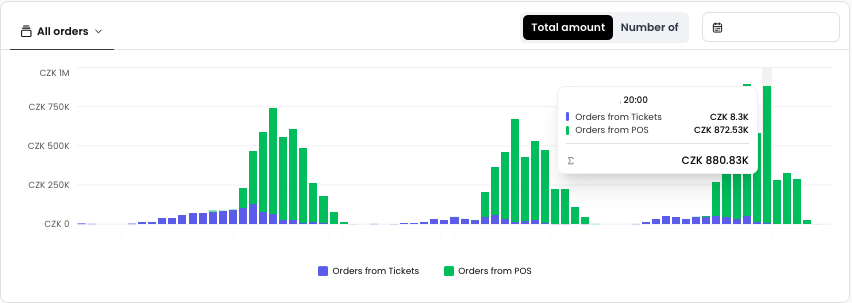
\includegraphics[width=\textwidth]{\ThesisFigures/ui/hub-chart-update}
		\caption{New Timeline Analysis in NFCtron Hub (December 2024 Update)}
		\label{fig:hub-chart-update}
	\end{figure}

	Also, thanks to the analytical findings and problems encountered during the analysis, I was able to provide valuable feedback to the development team.
	This will lead to improvements in the data collection process and the data model of the system, which will make future analysis easier and more efficient.

	Finally, the knowledge acquired by this thesis still shapes our product development and enables us to provide more advanced analytical capabilities to our clients – festival organizers.
	Future development will build upon these foundations, further expanding the analytical capabilities of NFCtron's system.
\end{section}